
Desoxyribonucleic Acid, commonly known as DNA~\cite{wiki:DNA} is the general medium of information common to all known living creatures. It defines the traits that all individuals from a species share, and thus, is the most important source of biological information for the understanding of life in general. This information is replicated when a cell goes under mitosis. It is the phase when a cell replicates its DNA and splits up to create two new cells. This ensures that the whole organism has a coherent DNA across all its cells.

DNA takes the form of two long string of proteins connected to each other to form a helical structure. These proteins are called "nucleotides" or "bases", as they are the base of the DNA code. There are four of them: adenine [A], thymine [T], cytosine [C] and guanine [G], often referred to by their first letter for ease of use. Adenine and thymine are linked together, and cytosine and guanine are also paired together, forming a double-helix, as shown in Figure~\ref{fig:double-stranded-dnamed}. This double-helix string is compacted in chromosomes, with an X-shape. Most animals are diploids, meaning they carry each chromosome twice, one from the mother and one from the father. Each species has its own number of chromosomes: for example, humans have 46 (23 pairs of chromosomes~\cite{ncbi:hg19}), cats have 38 (19 pairs~\cite{ncbi:cat}), and dogs have 78 (39 pairs~\cite{ncbi:dog}). The full DNA information of an individual is the genome of this individual.


\begin{figure}[h]
	\centering
	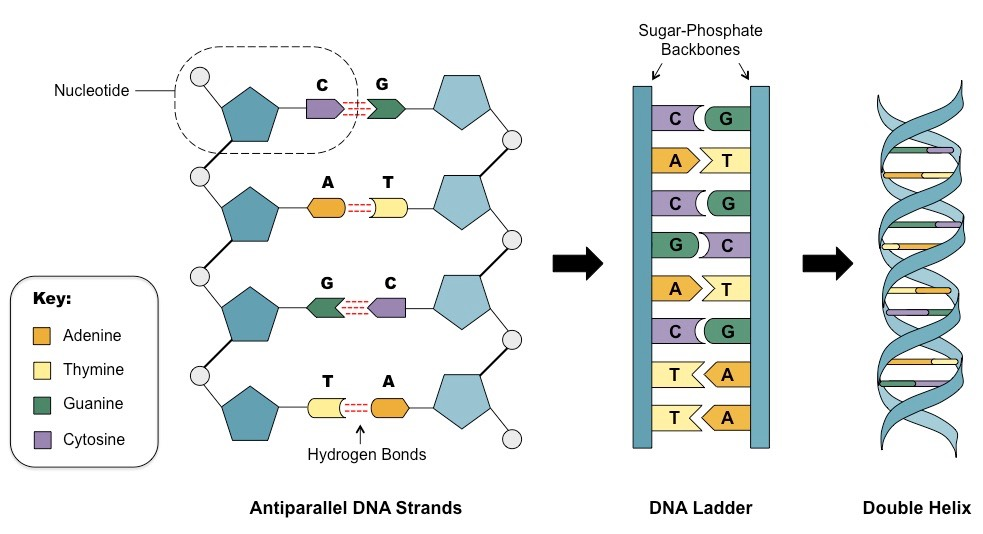
\includegraphics[width=1\linewidth]{double-stranded-dna_med}
	\caption{DNA double-helix with nucleotides (from~\cite{cornell:dnastructure})}
	\label{fig:double-stranded-dnamed}
\end{figure}


Inside a species, DNA can present small differences from one individual to another, in regions that are usually defining a variable trait (for example, hair colour). Portions of DNA defining a characteristic are called \emph{genes}, and there can be multiple viable variants of a gene. These variants are called \emph{allels}. Sexual reproduction is a key step to mix DNA from two individuals and create diversity among a species. These variations can be introduced at sexual reproduction. If the mutation gives the bearer an advantage in life over the non-bearers, it has a high probability to get passed to the bearer's descendants, fostering its propagation in the population (for example, having coloured petals for flowers makes them attractive for insects, and since coloured flowers have become more pollinated, their heirs will inherit this trait). On the contrary, if the mutation becomes a drawback, it is unlikely to be passed to the descendants.

Some DNA mutations are proven deadly, and the most well-known in this category is cancer~\cite{misc:diseases}. A cell whose DNA has been damaged or altered can start multiplying in an uncontrollable fashion, creating a pack of cells growing ever bigger, becoming malign and threatening the normal behaviour of an organ. This process, known as carcinoma, can be detected by multiple ways, some more empirical than others (for example, an easy setup with X-rays can allow a doctor to detect a small abnormal spot, which could be a sign of carcinoma). One way to detect this is by getting a sample of DNA from a patient, and comparing it with a known reference. \emph{Reference genomes} are build from a pool of donors: it is meant to be representative of a species' genes. In the case of the human genome sequences in 2009 "hg19", it has been put together from thirteen American individuals from Buffalo, NY~\cite{referencegenome}.
To achieve this comparison, one needs to find which area of the reference genome matches with the samples, or said differently, one needs to align the sample DNA with the reference and find how similar these two are.


% Consequently, we define a metric to quantify that closeness, called the \emph{alignment score}.

% In this case, only a pair of sequences are being matched: a sample, and a reference. This is called \emph{pairwise alignment}. Other cases where DNA alignment is needed can involve comparing multiple species' DNA to find regions that share some similarity, and that could translate into shared trait among species. In that situation, multiple sequences are mapped together, which makes it yet another problem.